\chapter{Histogram View}
\label{sec:histo_view}

A Histogram View displays the distribution of one numerical variable as a histogram, approximating the statistical distribution of said varable. When started, it presents itself in the following manner.

\begin{figure}[H]
    \hspace*{-2cm}
    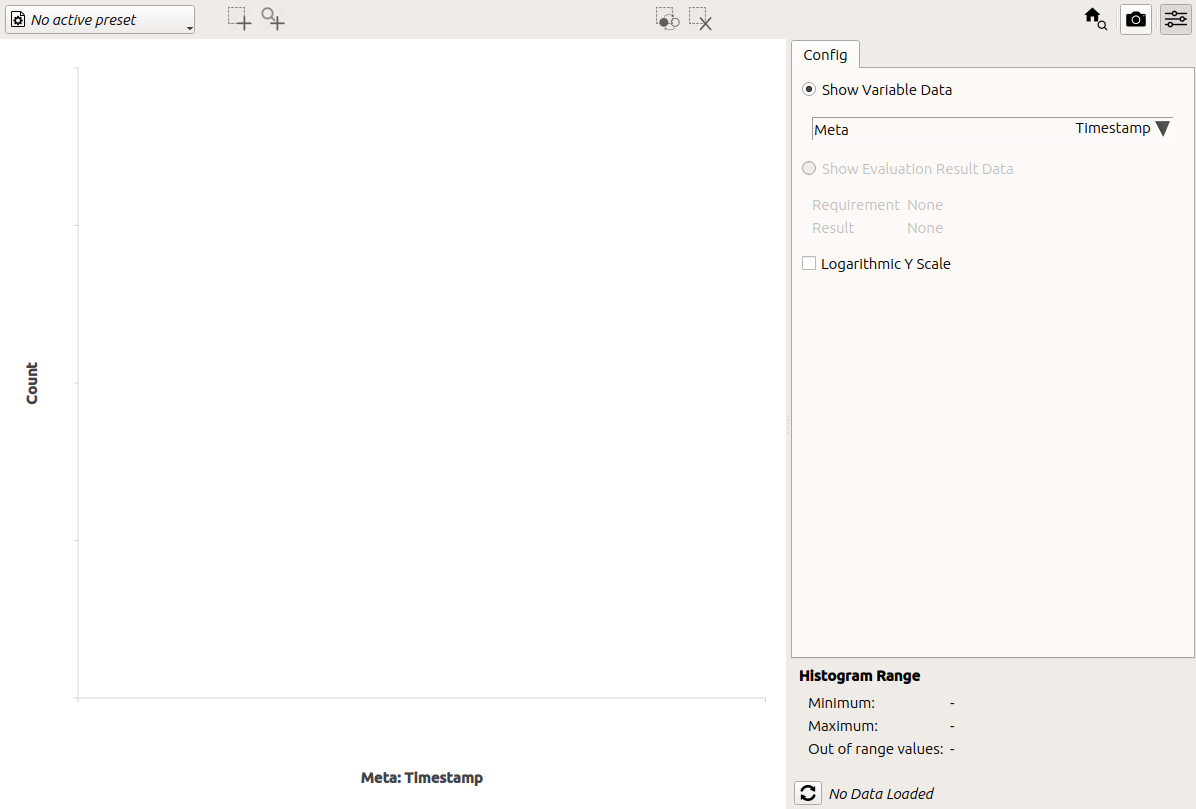
\includegraphics[width=18cm,frame]{figures/histogram_start.png}
  \caption{Histogram View startup}
\end{figure}

\section{Layout}

On the left side resides the plot area in which the histogram is shown (if data has been loaded). 
The tool bar at the top shows the currently selected tool and the available actions.\\

On the right side resides the configuration area, which allows configuring what data is loaded and how it is displayed.
The 'Reload' button on the bottom can be used to trigger a reload of the view's data.\\

Both areas can be resized and hidden if wanted.

\section{Data Loading}

To load the data the mechanism described in Section \nameref{sec:ui_overview} or the 'Reload' button can be used. To filter the dataset, the mechanism described in Section \nameref{sec:filters} can be used. \\

\begin{figure}[H]
    \hspace*{-2cm}
    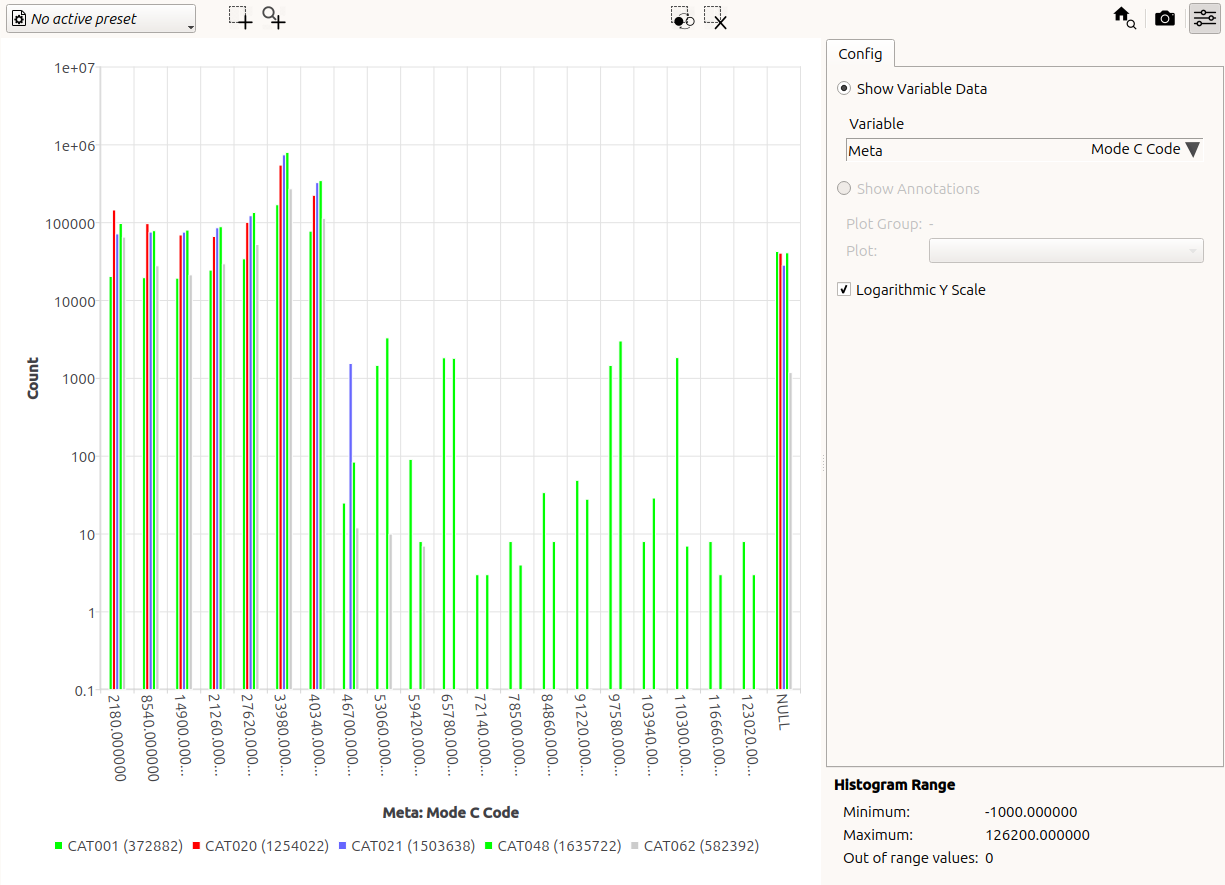
\includegraphics[width=18cm,frame]{figures/histogram_loaded.png}
  \caption{Histogram View after loading}
\end{figure}

On the x-axis the selected variable's data range is discretized into 20 bins. An additional bin represents all NULL values.
%plus one optional NULL value bin), scaled between the minimum and maximum value of the loaded data. 

On the y-axis the bin sizes per DBContent are shown, either in linear or logarithmic scale. \\

Below the histogram a legend is shown, giving the total counts of all data points. \\

% TODO_V7 Per DBContent - correct?
In the current example the meta-variable 'Timestamp' is used, showing the overall data rate per DBContent.

\section{Usage}

\subsection{Toolbar}

%TODO_V7 Maybe we could reformulate that, as only one button/mode is available after all?
The first button can be used to activate the selection tool (shortcut refers to keyboard shortcut). 

Note that an active tool can always be ended by pressing the 'Escape' key. 

\begin{table}[H]
  \center
  \begin{tabular}{ | l | l | l | l |}
    \hline
    \textbf{Icon} & \textbf{Shortcut} & \textbf{Text} & \textbf{Description} \\ \hline
    \includegraphics[width=0.5cm,frame]{../../data/icons/select_action.png} & S & Select & Allows data selection \& de-selection \\ \hline
  \end{tabular}
  \caption{Toolbar: Available tools}
\end{table}

%TODO_V7 Only refer to keyboard shortcuts when providing them
The others provide general operations.

\begin{table}[H]
  \center
  \begin{tabular}{ | l | l | l | l |}
    \hline
    \textbf{Icon} & \textbf{Shortcut} &\textbf{Text} &  \textbf{Description} \\ \hline
    \includegraphics[width=0.5cm,frame]{../../data/icons/select_invert.png} & & Invert Selection & Selects all de-selected \& vice versa \\ \hline
    \includegraphics[width=0.5cm,frame]{../../data/icons/select_delete.png} & & Delete Selection & De-selects all target reports \\ \hline
    %\includegraphics[width=0.5cm,frame]{../../data/icons/zoom_home.png} & Space & Zoom to Home & Pans/zooms to show all existing data \\ \hline
  \end{tabular}
  \caption{Toolbar: Available operations}
\end{table} 

\subsection{Config Tab}

The elements on the top define which data is visualized in the histogram. \\

Any numerical variable can be visualized by checking the 'Show Variable Data' box and selecting a variable in the selection control below.
A reload operation might be required for the selection to take effect. \\

Result data can be visualized by checking the 'Show Evaluation Result Data' box. 
In this case the the 'Requirement' and 'Result' fields indicate which evaluation result is presented. \\

The 'Logarithmic Y Scale' checkbox can be used to switch between linear and logarithmic scale of the y-axis. \\

\subsection{Histogram}

%\subsubsection{Zoom}

%The mouse wheel can be used to zoom in or out of the presented data. This is in the current presentation only useful in limited circumstances. The space key can be used to reset to the default zoom level (euqivalent to \includegraphics[width=0.5cm,frame]{../../data/icons/zoom_home.png}).

\subsubsection{Selection Tool}

If the 'Select' tool is active, data can be selected. Using the left mouse-button a red selection rectangle can be spanned across all bins that should be selected.

\begin{figure}[H]
    \hspace*{-2cm}
    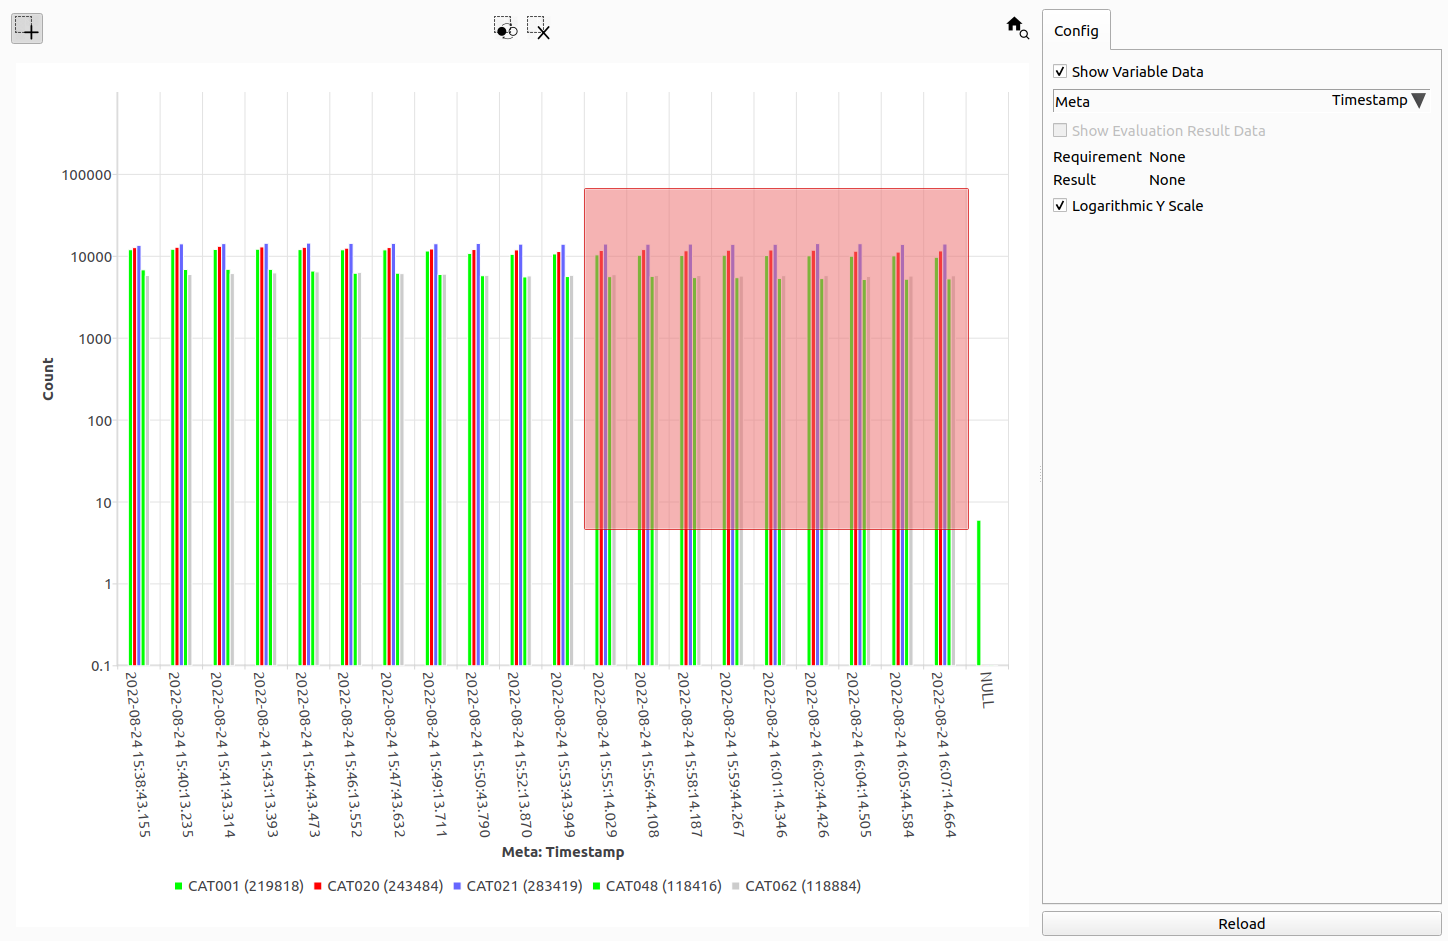
\includegraphics[width=18cm,frame]{figures/histogram_select.png}
  \caption{Histogram View data selection}
\end{figure}

The selected data is then presented in an extra 'Selected' entry in the legend, showing the count of all selected data points.

\begin{figure}[H]
    \hspace*{-2cm}
    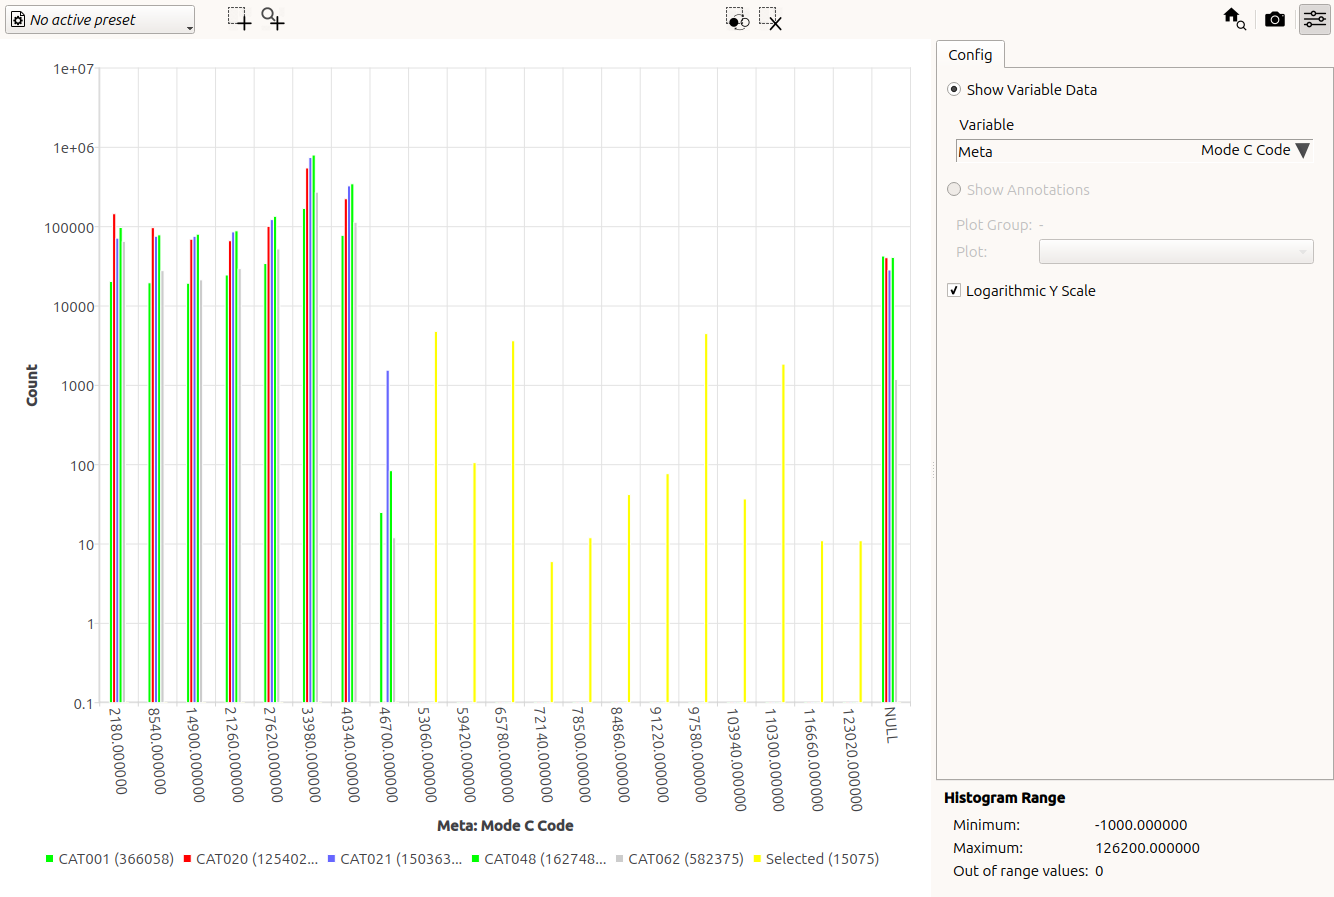
\includegraphics[width=18cm,frame]{figures/histogram_selected.png}
  \caption{Histogram View data selected}
\end{figure}

This enables selection of parts of the data based on the presented variable, allowing deeper analysis e.g. of dubious data. \\

The 'Invert Selection' \includegraphics[width=0.5cm,frame]{../../data/icons/select_invert.png} or 'Delete Selection' \includegraphics[width=0.5cm,frame]{../../data/icons/select_delete.png} actions allow for easier selection of the wanted target reports. \\

By pressing the 'Control' key while selecting, the newly selected data is added to any previous selection. This can be used to select data incrementally, making more complex selections possible.

\subsection{Evaluation Result}

If a requirement result is presented by using the Evaluation feature, the respective data is shown in the histogram.

%TODO_V7: Add updated evaluation figures
\begin{figure}[H]
    \hspace*{-2cm}
    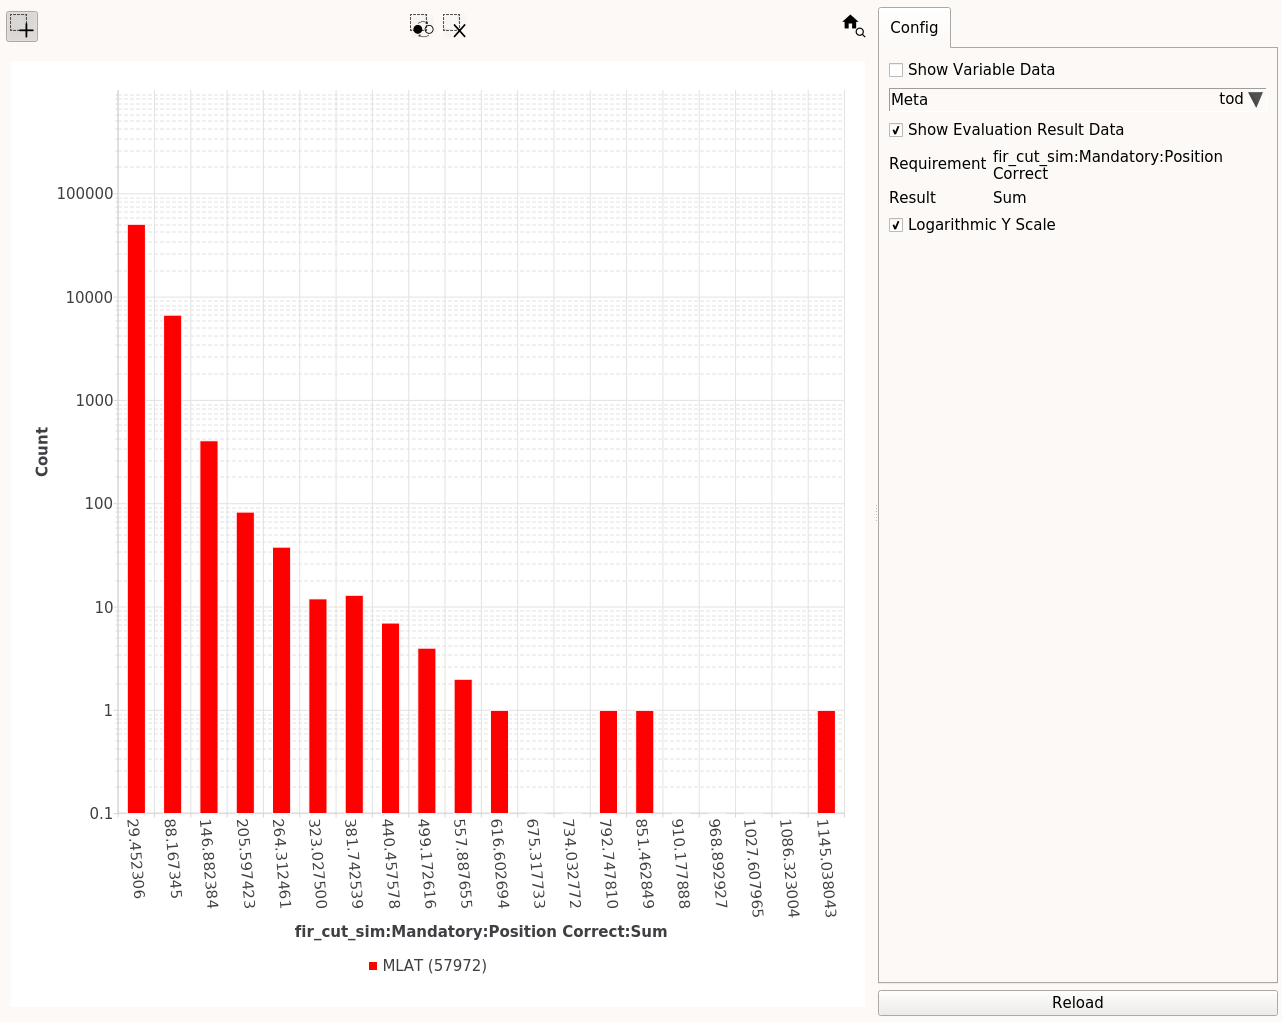
\includegraphics[width=18cm,frame]{figures/histogram_eval_pos_correct.png}
  \caption{Histogram View evaluation position correction result}
\end{figure}


\begin{figure}[H]
    \hspace*{-2cm}
    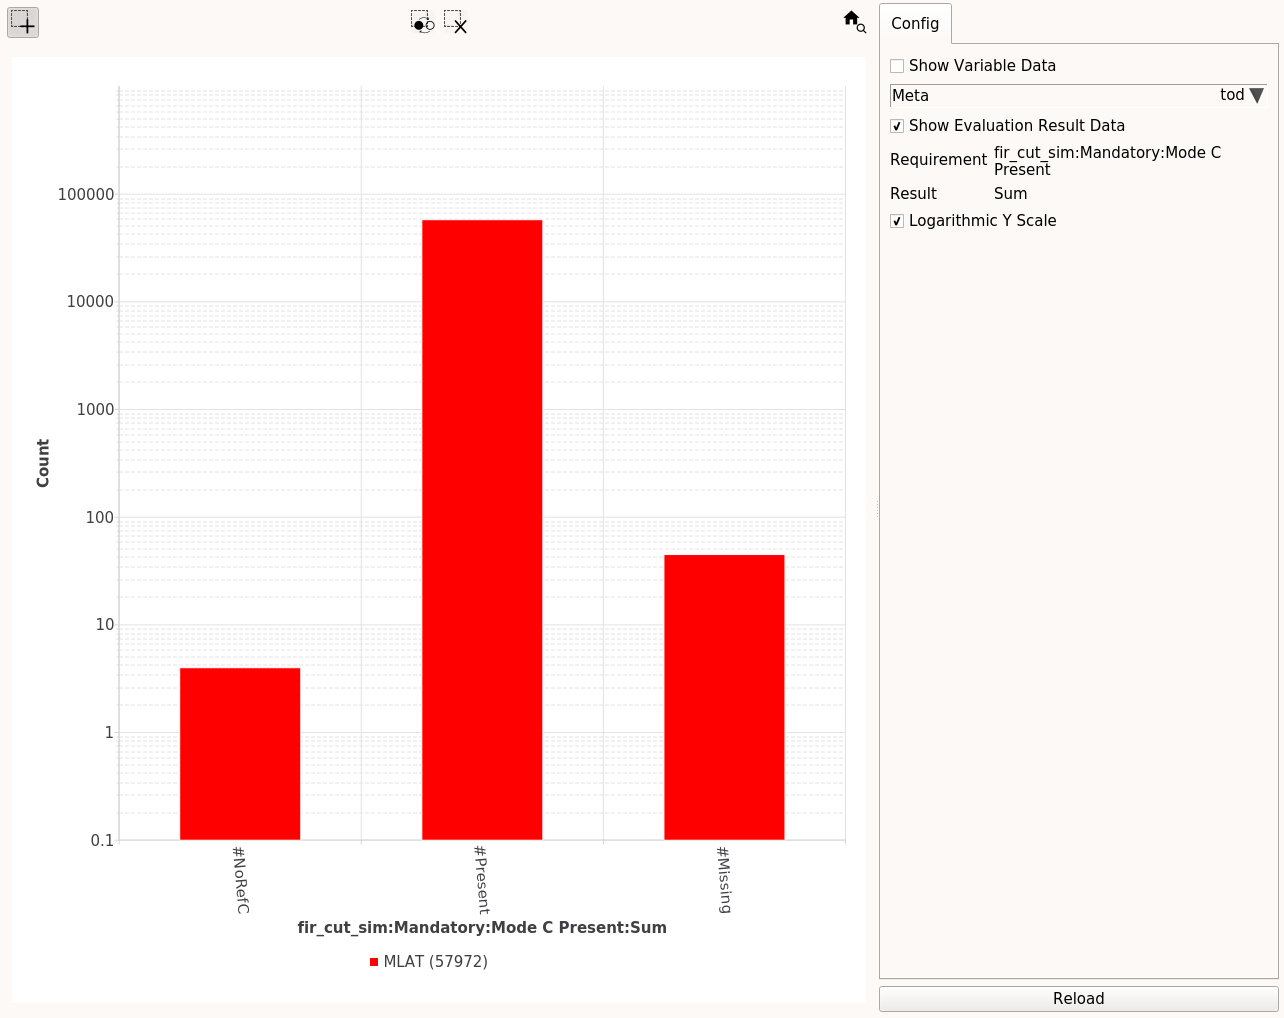
\includegraphics[width=18cm,frame]{figures/histogram_eval_mc.png}
  \caption{Histogram View Mode C present result}
\end{figure}

Please note that currently evaluation result data can not be selected. This will be improved in one of the next versions.
